% Harus dimuat terlebih dahulu, digunakan agar file PDF memiliki format karakter yang benar.
% Untuk informasi lebih lanjut, lihat https://ctan.org/pkg/cmap.
\RequirePackage{cmap}

% Format dokumen sebagai paper konferensi menggunakan aturan IEEEtran terbaru (v1.8b).
% Untuk informasi lebih lanjut, lihat http://www.michaelshell.org/tex/ieeetran/.
\documentclass[conference]{IEEEtran}[2015/08/26]

% Format encoding font dan input menjadi 8-bit UTF-8.
\usepackage[T1]{fontenc}
\usepackage[utf8]{inputenc}

% Format bahasa menjadi bahasa german dan inggris.
\usepackage[indonesian]{babel}

% Digunakan untuk tujuan demonstrasi.
\usepackage{mwe}

% Digunakan untuk menampilkan font dengan style yang lebih baik.
\usepackage[zerostyle=b,scaled=.75]{newtxtt}

% Digunakan untuk menampilkan tabel dengan style yang lebih baik.
\usepackage{booktabs}

% Digunakan untuk menampilkan gambar pada dokumen.
\usepackage{graphicx}

% Digunakan untuk menampilkan potongan kode.
\usepackage{listings}
\lstset{
  basicstyle=\ttfamily,
  columns=fixed,
  basewidth=.5em,
  xleftmargin=0.5cm,
  captionpos=b
}

% Digunakan agar backticks (`) dapat dirender pada PDF.
% Untuk informasi lebih lanjut, lihat https://tex.stackexchange.com/a/341057/9075.
\usepackage{upquote}

% Digunakan untuk menyeimbangkan bagian akhir dokumen dengan dua kolom.
\usepackage{balance}

% Digunakan untuk menampilkan pustaka.
\usepackage[square,comma,numbers,sort&compress]{natbib}

% Mengubah format ukuran teks pada natbib.
\renewcommand{\bibfont}{\normalfont\footnotesize}

% Menambah nama penulis ketika menggunakan perintah \citet.
% Untuk informasi lebih lanjut, lihat https://tex.stackexchange.com/a/76075/9075.
\usepackage{etoolbox}
\makeatletter
\patchcmd{\NAT@test}{\else \NAT@nm}{\else \NAT@hyper@{\NAT@nm}}{}{}
\makeatother

% Digunakan untuk melakukan linewrap pada pustaka dengan url yang panjang
% jika terdapat hyphens
\usepackage[hyphens]{url}

% Digunakan untuk menambah hyperlink pada referensi.
\usepackage{hyperref}

% Menonaktifkan warna dan bookmark pada hyperref.
\hypersetup{hidelinks,
  colorlinks=true,
  allcolors=black,
  pdfstartview=Fit,
  breaklinks=true
}

% Digunakan untuk membenarkan hyperref pada gambar.
\usepackage[all]{hypcap}

% Digunakan untuk menampilkan beberapa gambar
\usepackage[caption=false,font=footnotesize]{subfig}

\usepackage{stfloats}

% Tambahkan format tanda hubung yang benar di sini
\hyphenation{
  ro-ket
  me-ngem-bang-kan
  per-hi-tu-ngan
}

\begin{document}

  % Ubah kalimat berikut sesuai dengan judul penelitian.
\title{Prediksi Jumlah Kalori yang Terbakar saat Berolahraga dengan Treadmill Berbasis Kamera Menggunakan \emph{Convolutional Neural Network}}

% Ubah kalimat-kalimat berikut sesuai dengan nama, institusi, alamat dan kontak penulis.
\author{
  \IEEEauthorblockN{Dimas Aditya Maulana Fajri}
  \IEEEauthorblockA{\textit{Dept. Teknik Komputer}\\
  \textit{Institut Teknologi Sepuluh Nopember}\\
    Surabaya, Indonesia 60111\\
    dimas.adityamf@gmail.com}
  \and
  \IEEEauthorblockN{Eko Mulyanto Yuniarno}
  \IEEEauthorblockA{\textit{Dept. Teknik Komputer}\\
  \textit{Institut Teknologi Sepuluh Nopember}\\
    Surabaya, Indonesia 60111\\
    ekomulyanto@ee.its.ac.id}
  \and
  \IEEEauthorblockN{Arief Kurniawan}
  \IEEEauthorblockA{\textit{Dept. Teknik Komputer}\\
  \textit{Institut Teknologi Sepuluh Nopember}\\
    Surabaya, Indonesia 60111\\
    arifku@ee.its.ac.id} 
}

% Digunakan untuk menampilkan judul dan deskripsi penulis.
\maketitle

% Fakultas Teknologi Elektrodan Informatika Cerdas\\
%     Institut Teknologi Sepuluh Nopember\\
%     Surabaya, Indonesia 60111\\
%     dimas.adityamf@gmail.com}
  % Mengubah keterangan `Abstract` ke bahasa indonesia.
% Hapus bagian ini untuk mengembalikan ke format awal.
\renewcommand\abstractname{Abstrak}

\begin{abstract}

  % Ubah paragraf berikut sesuai dengan abstrak dari penelitian.
  Obesitas merupakan keadaan dimana terdapat penumpukan lemak pada tubuh seseorang yang menyebabkan berat badan berada pada nilai di atas normal. Ketidak seimbangan kalori yang dikonsumsi dan yang digunakan menyebabkan kelebihan berat badan. Salah satu aktivitas yang bisa mengurangi kelebihan berat badan adalah dengan olahraga yang memiliki kualitas aktivitas yang baik. Olahraga pada treadmill merupakan salah satu aktivitas yang dapat dilakukan dan melakukan pengukuran kalori yang terbakar. Namun perhitungan kalori pada treadmill masih belum akurat dan praktis. Penelitian ini membuat sistem yang dapat memprediksi kalori yang terbakar saat olahraga pada treadmill menggunakan citra video dengan kamera. Metode yang digunakan dengan melakukan pengambilan data yang kemudian dideteksi pose untuk postur tubuh. Model dibuat menggunakan CNN. Hasil deteksi berupa banyak langkah dan waktu untuk dilakukan prediksi kalori. Prediksi menggunakan regresi linear dan perhitungan MET. Hasil akhir yang diharapkan dapat memprediksi jumlah kalori yang terbakar dari citra video.

\end{abstract}

% Mengubah keterangan `Index terms` ke bahasa indonesia.
% Hapus bagian ini untuk mengembalikan ke format awal.
\renewcommand\IEEEkeywordsname{Kata kunci}

\begin{IEEEkeywords}

  % Ubah kata-kata berikut sesuai dengan kata kunci dari penelitian.
  Obesitas; kalori, prediksi, video.

\end{IEEEkeywords}


  % Ubah bagian berikut sesuai dengan konten-konten yang akan dimasukkan pada dokumen
  % Ubah judul dan label berikut sesuai dengan yang diinginkan.
\section{Pendahuluan}
\label{sec:pendahuluan}

% Ubah paragraf-paragraf pada bagian ini sesuai dengan yang diinginkan.

Penyakit tidak menular (PTM) meliputi penyakit kardiovaskular, kanker, penyakit pernapasan kronis dan diabetes telah menyebabkan kematian terhadap 41 juta orang setiap tahun dengan angka 74\% setara dengan nilai dari semua kematian secara global dan termasuk dalam penyebab utama kematian dan kecacatan dini. Indonesia memiliki angka kematian yang disebabkan oleh penyakit tidak menular sebesar 76\% dengan jumlah angka kematian sebanyak hampir 1,4 juta dan probabilitas kematian dini sekitar 25\% [1]. Faktor risiko utama dari terdiagnosis oleh penyakit tidak menular (PTM) adalah obesitas menyebabkan penurunan harapan hidup sekitar 5-20 tahun dengan melihat pada tingkat gangguan kondisi dan komorbid yang diderita [2]. Obesitas menjadi perhatian prioritas kesehatan global dalam mengatasi peningkatan tingkat kelebihat berat badan dan obesitas secara dini terhadap anak-anak dan remaja [3]. Obesitas dan penyakit gaya hidup menjadi perhatian dan masalah secara global [4].

Obesitas merupakan keadaan dimana terdapat akumulasi penumpukan lemak secara abnormal pada tubuh seseorang yang berlebihan dan menyebabkan berat badan pada nilai di atas normal yang dapat mengganggu kesehatan [5]. Indikasi yang dapat digunakan untuk menilai jika seseorang menderita kelebihan berat badan dan obesitas berdasarkan nilai body mass index (BMI) sebagai indek perbandingan berat badan dalam kilogram dengan kuadrat tinggi badan dalam meter [6]. Secara global nilai dari body mass index (BMI) memiliki tingkatan untuk kelebihan berat badan ditunjukkan dengan nilai lebih dari 25kg/m2 dan untuk tingkat obesitas ditunjukkan dengan nilai 30kg/m2 [7]. Keseimbangan energi dalam tubuh sangat penting karena penyebab obesitas dipengaruhi oleh kalori yang dikonsumsi tidak seimbang dengan kalori yang digunakan oleh tubuh [8]. Tingkat kebugaran yang rendah dan ketidakaktifan fisik dapat berdampak buruk pada kesehatan dan dapat menyebabkan penyakit kronis seperti diabetes dan penyakit kardiovaskular [9]. Salah satu yang dapat digunakan untuk mencegah obesitas dan meningkatkan kebugaran untuk mengurangi kelebihan berat badan adalah dengan melakukan olahraga.

Olahraga merupakan bentuk kegiatan kebugaran yang dilakukan sebagai kemampuan seseorang dalam memenuhi tuntutan fisik melalui kegiatan jasmani yang dilakukan secara terstruktur melibatkan pergerakan tubuh secara berulang-ulang [10]. Aktivitas fisik dengan melakukan olahraga dapat membantu dalam penurunan berat badan dan mengobati obesitas. Hubungan antara aktivitas fisik dan hasil kesehatan memiliki keterkaitan untuk meningkatkan kardiorespirasi dan kebugaran otot [11]. Kegiatan yang melibatkan aktivitas fisik dapat meningkatkan kesehatan pada individu dengan dapat meningkatkan kualitas hidup dari manfaat kesehatan jasmani pada tubuh [12]. Manfaat dari kesehatan jasmani dengan melakukan aktivitas fisik sangat membantu peluang untuk kesehatan fisik dan mental terhadap program pengobatan obesitas [13]. Aktivitas olahraga dinilai bermanfaat dan sesuai prosedur dengan melihat bagaimana kualitas olahraga yang dilakukan. Pengukuran kualitas aktivitas fisik dapat dilakukan berdasarkan jumlah energi yang dikeluarkan selama melakukan aktivitas fisik yang dengan International Physical Activity Questionnaire (IPAQ) telah digolongkan menjadi kategori rendah, sedang dan tinggi melihat nilai Metabolic Equivalent of Task yang dihasilkan dari perhitungan durasi dan frekuensi [14]. Jumlah energi yang dikeluarkan selama melakukan aktivitas olahraga akan berbeda-beda tergantung dari jenis aktivitas, durasi dan faktor fisik. Salah satu aktivitas olahraga yang dilakukan penelitian dalam meningkatkan kualitas aktivitas fisik untuk membantu penurunan berat badan dan obesitas adalah olahraga pada treadmill.

Treadmill digunakan dalam alat olahraga untuk dapat melakukan pergerakan tanpa berpindah tempat dan tidak dilakukan di atas tanah langsung. Alat ini juga digunakan dalam berbagai penelitian dan kebutuhan klinis [15]. Treadmil mudah digunakan karena dapat mengatur kontrol kecepatan pergerakan dengan melangkah yang dapat diatur dan membutuhkan sedikit ruangan [16]. Penggunaan treadmil terdapat berbagai jenis yang diantaranya dapat digunakan dengan kecepatan tetap dan kecepatan diri sendiri yang sangat bermanfaat untuk mengurangi neuromuskuler [17][18]. Berolahraga pada treadmill menghasilkan perbedaan yang tidak signifikan dalam hasil pembakaran energi dan kalori dengan melakukan olahraga tanpa treadmill yang membuat treadmill sangat digemari untuk digunakan sehari-hari [16].

Perkembangan teknologi pada pengembangan mengenai pengenalan aktivitas manusia mulai berkembang. Dalam beberapa tahun terakhir, pengenalan aktivitas manusia dengan menggunakan sensor pengukuran inersia berkembang dengan tanpa ada sensor melalui visi komputer yang lebih praktis [19]. Pengembangan ilmu visi komputer turut berkembang dengan pembelajaran mesin menggunakan \emph{deep learning} yang berkembang dalam visi komputer, pemrosesan bahasa maupun pengenalan gambar, video dan suara [20]. Munculnya ilmu \emph{deep learning} menjadi metode yang populer dalam melakukan pengenalan aktivitas yang dibantu dengan metode \emph{convolutional neural network} sebagai pembelajaran pengenalan aktivitas dengan menggunakan gambar berbabis pembelajaran mesin [21][22].

Aktivitas yang dilakukan pada treadmill dengan perhitungan pembakaran kalori hanya dapat dilakukan pada beberapa jenis treadmill yang memiliki sistem perhitungannya. Treadmill dengan sistem yang kompleks memungkinkan memiliki harga jual yang lebih tinggi dari treadmill yang sederhana. Sistem yang digunakan hanya bisa digunakan pada treadmill saja tanpa bisa terhubung satu sama lain antar alat. Hal ini membuat pengumpulan data dari setiap aktivitas yang dilakukan tidak tercatat dengan baik. Oleh karena itu, diperlukan sistem prediksi jumlah kalori yang terbakar yang lebih praktis dan mudah digunakan untuk berolahraga pada treadmill.


Pembahasan pada paper ini dimulai dengan pemaparan mengenai metode penelitian (Bagian \ref{sec:MetodePenelitian}).
Berdasarkan hal tersebut, kami menunjukkan penelitian dan pembahasan (Bagian \ref{sec:PenelitianPembahasan}).
Terakhir, didapatkan kesimpulan dari penelitian yang telah dilakukan (Bagian \ref{sec:kesimpulan}).

  % Ubah judul dan label berikut sesuai dengan yang diinginkan.
\section{Penelitian Terkait}
\label{sec:penelitianterkait}

% Ubah paragraf-paragraf pada bagian ini sesuai dengan yang diinginkan.

Beberapa penelitian lain pernah dilakukan seperti yang dirumuskan oleh \citet{newton1687} bahwa \lipsum[5]
Hasil tersebut kemudian menjadi persamaan \ref{eq:hukumpertama}.

% Contoh pembuatan persamaan ilmiah.
\begin{equation}
  \label{eq:hukumpertama}
  \sum \mathbf{F} = 0\; \Leftrightarrow\; \frac{\mathrm{d} \mathbf{v} }{\mathrm{d}t} = 0.
\end{equation}

\lipsum[6-7]

  % Ubah judul dan label berikut sesuai dengan yang diinginkan.
\section{Arsitektur}
\label{sec:arsitektur}

% Ubah paragraf-paragraf pada bagian ini sesuai dengan yang diinginkan.

\subsection{Cetak Biru Roket}
\label{subsec:cetakbiruroket}

Pada cetak biru yang tertera pada Gambar \ref{fig:cetakbiru}. \lipsum[8]

% Contoh input gambar pada kolom.
\begin{figure} [ht]
  \centering
  % Ubah sesuai dengan nama file gambar dan ukuran yang akan digunakan.
  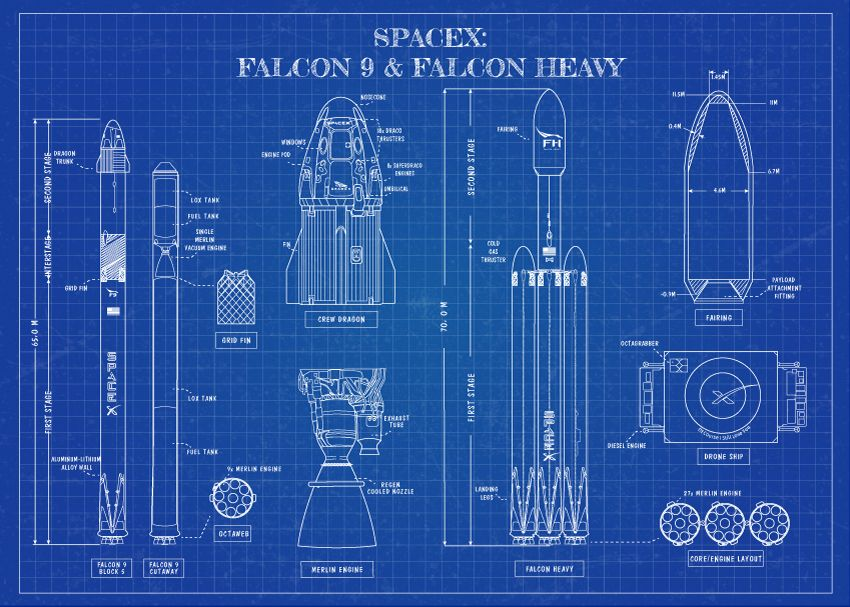
\includegraphics[width=0.4\textwidth]{gambar/cetakbiru.jpg}

  % Ubah sesuai dengan keterangan gambar yang diinginkan.
  \caption{Cetak biru roket yang akan diuji coba. \cite{cetakbiruspacex}}
  \label{fig:cetakbiru}
\end{figure}

\lipsum[9-10]

\subsection{Lorem Ipsum}
\label{subsec:loremipsum}

\lipsum[11]

% Contoh pembuatan tabel.
\begin{table}
  \caption{Contoh tabel sederhana}
  \label{tab:tabelsederhana}
  \centering
  \begin{tabular}{lll}
    \toprule
    Heading1 & Heading2 & Heading3  \\
    \midrule
    One      & Two      & Three     \\
    Four     & Five     & Six       \\
    \bottomrule
  \end{tabular}
\end{table}

% Contoh pembuatan potongan kode.
\begin{lstlisting}[
  language=C++,
  caption={Program halo dunia.},
  label={lst:halodunia}
]
#include <iostream>

int main() {
    std::cout << "Halo Dunia!";
    return 0;
}
\end{lstlisting}

\lipsum[12]

% Contoh pembuatan daftar.
\begin{enumerate}
  \item \lipsum[13][1-4]
  \item \lipsum[13][5-8]
  \item \lipsum[13][9-12]
\end{enumerate}

\lipsum[14-15]

  % Ubah judul dan label berikut sesuai dengan yang diinginkan.
\section{Lorem ipsum}
\label{sec:loremipsum}

% Ubah paragraf-paragraf pada bagian ini sesuai dengan yang diinginkan.

% Contoh input beberapa gambar pada halaman.
\begin{figure*}
  \centering
  \subfloat[Hasil A]{\includegraphics[width=.4\textwidth]{example-image-a}
    \label{fig:hasila}}
  \hfil
  \subfloat[Hasil B]{\includegraphics[width=.4\textwidth]{example-image-b}
    \label{fig:hasilb}}
  \caption{Contoh input beberapa gambar.}
  \label{fig:hasil}
\end{figure*}

\lipsum[16-18]

% Contoh input potongan kode dari file.
\lstinputlisting[
  language=Python,
  caption={Program perhitungan bilangan prima.},
  label={lst:bilanganprima}
]{program/bilangan-prima.py}

\lipsum[19-20]

  % Ubah judul dan label berikut sesuai dengan yang diinginkan.
\section{Kesimpulan}
\label{sec:kesimpulan}

% Ubah paragraf-paragraf pada bagian ini sesuai dengan yang diinginkan.

\lipsum[21-23]


  % Menampilkan daftar pustaka dengan format IEEE
  \bibliographystyle{IEEEtranN}
  \bibliography{pustaka/pustaka.bib}

  % Menyeimbangkan bagian akhir di kedua kolom
  \balance

\end{document}
